\documentclass{article}
\usepackage[top=1.5cm,left=2cm, right=2cm, bottom=2cm]{geometry}
\usepackage[T1]{fontenc}
\usepackage[utf8]{inputenc}
\usepackage{lmodern}
\usepackage[english]{babel}
\usepackage{graphicx}
\usepackage{geometry}
\usepackage{physics}
\usepackage{caption}
\usepackage{subcaption}
\usepackage[round]{natbib}
\usepackage{amsmath,amssymb}
\usepackage{mathtools}
\usepackage{xcolor}
\usepackage{listings}
\usepackage{hyperref}
\hypersetup{
    colorlinks=true,
    linkcolor=blue,
    filecolor=magenta,      
    urlcolor=cyan,
    citecolor=blue,
}
\setlength{\parindent}{0pt}
\usepackage{aastex}
\usepackage{array}
\newcolumntype{L}{>{$}l<{$}}
\newcolumntype{R}{>{$}r<{$}}
\newcolumntype{C}{>{$}c<{$}}

\definecolor{blazeorange}{rgb}{1.0, 0.6, 0.2}
\definecolor{seagreen}{rgb}{0.18, 0.55, 0.34}
\definecolor{rufous}{rgb}{0.66, 0.11, 0.03}
\definecolor{royalfuchsia}{rgb}{0.79, 0.17, 0.57}
\definecolor{scarlet}{rgb}{1.0, 0.13, 0.0}
\definecolor{royalpurple}{rgb}{0.47, 0.32, 0.66}
\definecolor{darkblue}{rgb}{0, 0, 0.66}
\definecolor{violet}{rgb}{0.5,0.,0.5}

%% COMMENTS AND CORRECTIONS/CHANGES %%
\newcommand\jg[1]{{\color{royalfuchsia}[JG: #1]}}
\newcommand\jgcor[1]{{\color{royalfuchsia}#1}} 
\renewcommand\pb[1]{{\color{seagreen}[[[PB: #1]]]}}
\newcommand\pbcor[1]{{\color{seagreen}#1}}
\newcommand\add[1]{{\color{orange}#1}}

\newcommand{\on}{{\rm on}}
\newcommand{\off}{{\rm off}}
\newcommand{\sh}{{\rm sh}}
\newcommand{\pk}{{\rm pk}}
\newcommand{\bk}{{\rm bk}}
\newcommand{\bol}{{\rm bol}}
\newcommand{\rise}{{\rm rise}}
\newcommand{\HLE}{{\rm HLE}}
\newcommand{\eff}{{\rm eff}}
\newcommand{\RS}{{\rm RS}}
\newcommand{\FS}{{\rm FS}}

\title{Fitting prompt GRB pulses}
\author{A. Charlet, J. Granot}
\date{May 2026}

\begin{document}

\maketitle

This document serves as a documentation for the modeling of peak frequency and flux of a pulse in the internal shock model in spherical geometry, based on analytical work of \cite{rahaman2024internal, rahaman2024prompt} (R24a,b) and numerical simulations of \cite{charlet2025numerical} (C25). The shock emits radiation while propagating in the shell then turns off once it has fully crossed. %\textbf{Edit 11/05/2026:} changed the physical fit parameter $\Delta R/R_0$ to $\tau\equiv t_\on/t_\off$, added calculation of the FS, added spectral model for time-resolved fits, updated Python script accordingly. \textbf{Edit 27/05/2026:} corrected equations \ref{eqn:TfRS} and \ref{eqn:TfFS}, added description of spherical effects and method

\section{Model}\label{sec:model_R24}
This model produces the evolution of normalized peak flux with normalized peak frequency from a shock front, assuming the shells propagate with ultra-relativistic velocities. It only needs two input parameters to fully determine this evolution (three inputs for both shock fronts):
\begin{itemize}
    \item the proper velocity contrast between the shells: $a_u$,
    \item the ratio of activity time (duration of the shell emission) over inactivity time (duration between the emission of the two shells) of the source, $\tau\equiv t_\on/t_\off$. This ratio can also be interpreted as the initial width of the shell before collision normalized to the collision radius, and is directly linked to the crossing time in the observers frame, $T_f$.
\end{itemize}
The proper velocities contrast $a_u$ determines most of the physics in this context, in particular the Lorentz factor ratio $g=\Gamma_d/\Gamma_\sh$ of the emitting material to the shock front, and the link between the contributions of each shock front. Then, a full spectral model is built from the evolution of the peaks by adding a spectral shape (typically a Band function), and the normalizations of time, energy, and flux.

In this section, the Lorentz factors of the shock fronts and emitting regions do not evolve during propagation, implying the rate of energy dissipation behind each front also stays constant. In the comoving frame of the emitting regions, peak frequency is taken to evolve with $R^{-1}$. We add effects from evolving Lorentz factors with propagation in \S\,\ref{sec:spherical}.

\subsection{Peak frequency and peak flux}\label{sec:pks_R24}
We define the normalized time $\tilde{T}_{\rm eff,1}$ (see Appendix H of R24b), which we use to express the normalized peak frequency and flux during the rising part of the pulse:
\begin{align}
    &\tilde{T}_{\rm eff,1} = (1-g^2) + g^2 \tilde{T},\\
    &\tilde{\nu}_{\pk,\rise}(\tilde{T}) = \tilde{T}^{-1},\label{eqn:nupk_R24}\\
    &(\widetilde{\nu F_\nu})_{\pk,\rise}(\tilde{T}) = 1 - \tilde{T}_{\rm eff, 1}^{-3}.\label{eqn:nFpk_R24}
\end{align}
We note $\tilde{\nu}\equiv\nu/\nu_0$ and $\widetilde{\nu F_\nu}\equiv\nu F_\nu/\nu_0F_0$. $\tilde{T}\equiv 1 +(T-T_s)/T_{0,\sh}$ is the time in the observer frame, measured from the arrival of the first emitted photon $T_s$ and normalized to $T_{0,\sh}$ the shock front angular time at collision radius. After a time $T_f$ corresponding to the arrival time of the first photon emitted when the shock fully crossed the shell, emission stops in the source frame and we start observing contributions from the high-latitude regions of the shell. We define a second normalized time $\tilde{T}_{\rm eff,2}$ and express the peak frequency and flux as:
\begin{align}
    &\tilde{T}_{\rm eff,2} = (1-g^2) + g^2 \frac{\tilde{T}}{\tilde{T}_f},\\
    &\tilde{\nu}_{\pk,\HLE}(\tilde{T}) = \tilde{\nu}_{\pk,\rise}(\tilde{T}_f)\,\tilde{T}_{\rm eff,2}^{-1},\label{eqn:nupk_HLE}\\
    &(\widetilde{\nu F_\nu})_{\pk,\HLE}(\tilde{T}) = (\widetilde{\nu F_\nu})_{\pk,\rise}(\tilde{T}_f)\,\tilde{T}_{\rm eff,2}^{-3}.\label{eqn:nFpk_HLE}
\end{align}
Then, noting $\nu_\bk\equiv\nu_{\pk,\rise}(T_f)$ and $(\nu F_\nu)_\bk\equiv (\nu F_\nu)_{\pk,\rise}(T_f)$, we get the correlation (for one front):
\begin{equation}
(\widetilde{\nu F_\nu})_\pk(\tilde{\nu}_\pk) = \begin{cases}
        1 - \left[(1-g^2) + g^2\tilde{\nu}_\pk^{-1}\right]^{-3}&\tilde{\nu}_\pk\geq\tilde{\nu}_\bk\\
        (\widetilde{\nu F_\nu})_\bk\left(\dfrac{\tilde{\nu}_\pk}{\tilde{\nu}_\bk}\right)^3&\tilde{\nu}_\pk<\tilde{\nu}_\bk
    \end{cases}\label{eqn:pk_corr}
\end{equation}
\textbf{N.B.:} a 'renormFlux' is set to true by default in the code. It causes the peak flux to be given in units of the max peak flux $(\widetilde{\nu F_\nu})_\bk$ (an observable) rather than in units $F_0$ which cannot be physically measured in the data.

\subsection{From source parameters to observed quantities}\label{sec:ratios}
\subsubsection{Lorentz factors ratios}
The ratios $g_\RS\equiv\Gamma_3/\Gamma_\RS$ and $g_\FS\equiv\Gamma_2/\Gamma_\FS$ can be determined from $a_u$ by plugging Eqn. (A4) of R24b in Eqns. (C2) and (C5) of R24a:
\begin{align}
    &K_u \equiv \left(\frac{2}{1+a_u^2}\right)^{1/2},\\
    &\Gamma_{34}=\frac{1}{2}\left(K_u+K_u^{-1}\right),\quad\Gamma_{21}=\frac{1}{2}\left(K_u a_u+(K_u a_u)^{-1}\right),\label{eqn:relLfacs}\\
    &g_\RS^2=\frac{4\Gamma_{34}-K_u}{4\Gamma_{34}-K_u^{-1}},\quad g_\FS^2=\frac{a_uK_u-4\Gamma_{21}}{(a_uK_u)^{-1}-4\Gamma_{21}}.\label{eqn:g2_from_au}
\end{align}
\textbf{N.B.:} in this context, $\Gamma_2=\Gamma_3=K_ua_u\Gamma_1=K_u\Gamma_4$.

\subsubsection{Break times}\label{sec:Tf_R24}
The break time $T_f$ from a front is related to the activity time ratio $\tau=t_\on/t_\off$ of its shell by deriving the distance crossed by the shock front during its emission lifetime $\Delta R_\sh$:
\begin{equation}
\begin{split}
    &\tilde{T}_{f,\RS} = 1 + \frac{\Delta R_\RS}{R_0} = 1 + \left[\frac{2(a_u^2-1)}{(a_u^2+1)g_\RS^2-2}\right]  \tau_4,\\
    &\tilde{T}_{f,\FS} = 1 + \frac{\Delta R_\FS}{R_0} = 1 + \left[\frac{2(a_u^2-1)}{2 a_u^2 - (a_u^2+1)g_\FS^2}\right] \tau_1.
\end{split}\label{eqn:Tf_from_tau}
\end{equation}
\textbf{N.B.:} $\tilde{T}_{f,\RS}$ is in units $T_{0,\RS}$ and $\tilde{T}_{f,\FS}$ in units $T_{0,\FS}$.

\subsubsection{Ratios of normalizations between the shocks}\label{sec:norm_ratios}
Assuming a constant and equal source luminosity during the emission of both shells, the ratios of angular time, peak frequency, and flux normalizations of both shocks fronts are a function of $a_u$ only:
\begin{align}
    &\frac{T_{0,\RS}}{T_{0,\FS}}\approx \frac{\Gamma_\FS^2}{\Gamma_\RS^2} = \frac{g_\RS^2}{g_\FS^2},\label{eqn:ratio_T}\\
    &\frac{\nu_{0,\RS}}{\nu_{0,\FS}} = \left(\frac{\Gamma_{34}+1}{\Gamma_{21}+1}\right)^{-1/2}\left(\frac{\Gamma_{34}}{\Gamma_{21}}\right)^{1/2}\left(\frac{\Gamma_{34}-1}{\Gamma_{21}-1}\right)^2,\label{eqn:ratio_nu}\\
    &\frac{F_{0,\RS}}{F_{0,\FS}}=\frac{\epsilon_{\rm rad,\RS}}{\epsilon_{\rm rad,\FS}}\left(\frac{\Gamma_{34}+1}{\Gamma_{21}+1}\right)^{-1/2}\left(\frac{\Gamma_{34}}{\Gamma_{21}}\right)^{1/2}\left(\frac{\Gamma_{34}-1}{\Gamma_{21}-1}\right)^{-2}\frac{\beta_{34}}{\beta_{21}}.\label{eqn:ratio_F}
\end{align}
$\epsilon_{\rm rad,\sh}$ is the radiative efficiency of emission at a shock front. By default, we consider both shocks to be in the (very) fast synchrotron cooling regime, $\epsilon_{\rm rad,\RS}=\epsilon_{\rm rad,\FS}=1$, but the radiative efficiency of the FS can be changed as a free parameter. 

\subsection{Time binning}\label{sec:tbin}
Even when performing 'time-resolved' spectroscopy when a pulse is bright enough, we're truly looking at time-integrated spectra over small time bins. Thus, the model needs to output peak frequency and flux over time-integrated spectra. Instead of computing full flux and finding maximal peak energy and flux, the code perform these:
\begin{align}
    &\langle \tilde{\nu}_\pk \rangle =  \frac{\displaystyle\int_{\tilde{T}_1}^{\tilde{T}_2}(\widetilde{\nu F_\nu})_\pk(\tilde{T})}{\displaystyle\int_{\tilde{T}_1}^{\tilde{T}_2} \tilde{F}_\pk(\tilde{T}){\rm d}\tilde{T}},\\
    &\langle (\widetilde{\nu F_\nu})_\pk \rangle = \int_{\tilde{T}_1}^{\tilde{T}_2} \tilde{F}_\pk(\tilde{T}){\rm d}\tilde{T}.
\end{align}
The error introduced by this method compared to full full computation is of order a few \% ($\lesssim5$\% in $\nu F_\nu$, $\lesssim2$\% in $\nu$) only in the worst case scenario where the bin starts at the beginning and contains the full pulse and part of the HLE ($\Delta\tilde{T}=3$ in the $a_u=2$ and $\tau=1$ fiducial case). For a 'small' bin of $\Delta \tilde{T}<1$, these errors are $\lesssim 0.5$\%. These integrals are performed by trapezoidal rule over 20 bins. This binning is especially important for the first(s) time bins were the peak energy and peak flux varies greatly over the bin. In particular the peak energy in the first bin is not $\nu_0$ and, this binning allows for a more accurate placement of these first bins on the correlation track. 

\subsection{Spectral model}
The missing ingredient for a full determination of the observed flux is the spectral shape at each emission front. We choose to model each component by a Band function with slopes from synchrotron theory, assuming we're deep in the fast cooling regime: $(\alpha, \beta)=(-1/2, -p/2)$, with $p$ the index of the non-thermal electron distribution:
\begin{equation}
S[x;\alpha,\beta] = e^{1+\alpha}\begin{cases}
    x^{1+\alpha}e^{-(1+\alpha)x} &x\leq x_{\rm b},\\
    x^{1+\beta}x_{\rm b}^{\alpha-\beta}e^{-(\alpha-\beta)} &x\geq x_{\rm b},
\end{cases}
\end{equation}
with $x_{\rm b}=(\alpha-\beta)/(1+\alpha)$. Finally, the observed flux is modeled by:
\begin{equation}
F_\nu(T) = \sum_{i=\RS,\FS} F_{0,i} \tilde{F}_{\pk,i}(\tilde{T}_i;a_u,\tau_i) S\left[\frac{\nu}{\nu_{0,i}\tilde{\nu}_{\pk,i}(\tilde{T}_i;a_u,\tau_i)};\alpha_i,\beta_i\right].
\end{equation}
By default, $\alpha_\RS=\alpha_\FS$ and $\beta_\RS=\beta_\FS$, but it is possible to leave them as free parameters. For instance, on can choose the weaker FS to be in the marginally fast cooling regime \citep[see e.g.][]{beniamini2018marginally}, invoked to explain successful GRB prompt fits with a synchrotron-like doubly broken power law \citep[e.g.][]{ravasio2019evidence}. In that case $\epsilon_{\rm rad,\FS}=1/2$ and $\alpha_\FS=1/3$.

\subsection{Normalizations and physical parameters}
The shape of the correlation is a function of two parameters only, but the complete model predicts the normalizations with more parameters. I present here the formula for the collision radius $R_0$, and the angular time, peak frequency and flux normalizations, $T_0$, $\nu_0$ and $\nu_0 F_0$, for the reverse shock. The corresponding normalizations for the forward shock are obtained using the ratios given in \S \ref{sec:norm_ratios}. Their full derivation can be found in appendix (G) of R24b.
\begin{align}
    R_0 &= \frac{\beta_1\beta_4ct_{\rm off}}{\beta_4 - \beta_1}\approx\frac{2u_1^2ct_{\rm off}}{1-a_u^{-2}},\\
    T_{0,\RS} &= (1+z) \frac{R_0}{c}\frac{1-\beta_\RS}{\beta_\RS} \approx (1+z) \frac{R_0}{2c\Gamma_\RS^2} = (1+z) \left(\frac{g_\RS}{2}\right)^2\frac{a_u^2+1}{a_u^2-1}t_\off,\\
    \nu_{0,\RS} &= \frac{1}{(1+z)}\left[\frac{2}{\pi}\frac{q_{\rm e} m_{\rm p}^2}{m_{\rm e}^3c^{5/2}}\right]\left(\frac{p-2}{p-1}\right)^2\xi_{\rm e}^{-2}\epsilon_{\rm e}^2\epsilon_{\rm B}^{1/2}\left[\Gamma_{34}^{1/2}(\Gamma_{34}-1)^{5/2}\frac{1-a_u^{-2}}{\sqrt{1+a_u^2}}\right]u_1^{-1}L^{1/2}t_{\rm off}^{-1},\\
    (\nu_0 F_0)_\RS &= \frac{4}{9\pi d_L^2}\frac{p-2}{p-1}\frac{(\Gamma_{34}-1)u_{34}}{1+a_u^2}\epsilon_{\rm e}\epsilon_{\rm rad,\RS}L.
\end{align}
We give Table \ref{tab:parameters} a summary of the physical parameters of the model. With the fiducial values given in this table, assuming a redshift $z=1$ and a luminosity distance $d_L=2\times10^{28}$ cm, we get $T_{0,\RS}=0.22$ s, $h\nu_{0,\RS}=450$ keV, and $(\nu_0 F_0)_\RS=4\times10^{-8}$ erg.s$^{-1}$.cm$^{-2}$.
\begin{table}[ht!]
\centering
\caption{Physical parameters}
\begin{tabular}{|C|c|l|}
\hline
  & Fiducial value & Physical meaning\\\hline
L & $10^{53}$ erg/s & Source power\\
a_u\equiv u_4/u_1 & 2 & Proper velocities ratio\\
u_1\equiv\beta_1\Gamma_1 & 100 & Proper velocity of shell 1\\
\tau_1\equiv t_{\on,1}/t_\off & 1 & Activity timescale of shell 1 to inactivity timescale\\
\tau_4\equiv t_{\on,4}/t_\off & 1 & Activity timescale of shell 4 to inactivity timescale\\
t_\off & 0.1 s & Time between the emission of the shells\\\hline
p & 2.5 & Power-law index of the accelerated electrons distribution\\
\epsilon_e & 1/3 & Portion of the internal energy given to the accelerated electrons\\
\xi_e & $10^{-2}$ & Fraction of accelerated electrons\\
\epsilon_B & 1/3 & Portion of the internal energy given to the magnetic field \\\hline
\end{tabular}
\label{tab:parameters}
\end{table}

\section{Spherical effects}\label{sec:spherical}
In \cite{charlet2025numerical}, we identified effects of spherical geometry already present at $R\gtrsim R_0$ that were unaccounted for in R24a,b. In particular, the Lorentz factor of the shock fronts $\Gamma_\sh$ and of the downstream emitting material $\Gamma_d$ (their ratio $g$ staying very close to constant during shell propagation, equal to the analytical prescription) evolve with propagation, following an initial power-law segment that smoothly converges to a constant value. This evolution has a important impact on the hard-to-soft evolution of the emitted flux during the rise of the light curve, before transitioning to the high-latitude emission. We model this evolution with the function:
\begin{equation}
    f_Q(x) = A \left(\frac{x}{x_b}\right)^{-\alpha}\left\{\frac{1}{2}\left[1+\left(\frac{x}{x_b}\right)^{1/s}\right]\right\}^{(\alpha-\beta)s},\label{eqn:smooth_bpl}
\end{equation}
where we set $\beta=0$. Following this, we also model the quantities $\nu'_m$\footnote{In the data analysis we actually fit $\nu'_m\times R/R_0$ by the function with $\beta=0$ and later divide by $x$, rather than setting $\beta=1$ in the fit.} and $L'_\bol$ behind each front with the same function\footnote{All these functions can be obtained from $f_\Gamma(x)$ alone, but the current iteration of this method is a bit unsatisfactory.}. We explore the parameter space $\log(a_u-1)\in[-1,\,1.5]$ in increments of 0.1 by performing numerical simulations. For each simulation we fit these three\footnote{We actually fit four: $(\Gamma_{ud}-1)/(\Gamma_{ud,0}-1)$ is also fitted by $f_Q(x)$, which we use to reconstruct hydrodynamical data without numerical artifacts. The flux from which we extract the spectral peaks is computed from this reconstructed hydro data.} quantities, normalized to their theoretical expectation following R24a,b, with the function defined in Eqn. \ref{eqn:smooth_bpl}.

Following the approach introduced in C25, we model the peak frequency and flux at peak frequency of a given shock front by:
\begin{align}
    &\tilde{\nu}_\pk = \frac{f_\Gamma(x_\eff)f_{\nu'}(x_\eff)}{1+\xi_\eff},\label{eqn:nupk_C25}\\
    &(\widetilde{\nu F}_\nu)_\pk = 3\xi_{\max}  \left(\frac{f_\Gamma(x_\eff)}{1+\xi_\eff}\right)^4\frac{f_{L'_\bol}(x_\eff)}{f_\Gamma(x_L)^2},\label{eqn:nFpk_C25}
\end{align}
where we assume that the peak contribution at any given observer time $T$ corresponds to an effective radius $R_\eff(T)$ on the EATS. The functions $f_\Gamma$, $f_{\nu'}$, and $f_{L'_\bol}$ are defined by the fitting defined in the previous paragraph. We parametrize the EATS with the variable $\xi=(\Gamma\theta)^2$, $\xi_{\max}$ is thus the 'size' of the EATS in this variable ($\xi=0$ on the line of sight), and we chose to parametrize $\xi_\eff$ as a constant fraction $0\leq k_\xi\leq1$ of $\xi_{\max}$:
\begin{equation}
    \xi_{\rm eff} = k_\xi \xi_{\max} = k_\xi \left[\left(g^2(\tilde{T}-1)\right)^{-s}+\xi_{\rm sat}^{-s} \right]^{-1/s},\label{eqn:xieff}
\end{equation}
where $\xi_{\rm sat}$ is a constant value to account for the Doppler beaming that severely inhibits any contribution coming from angles $\theta>1/\Gamma_d$. The parameters $k_\xi$, $\xi_{\rm sat}$ and $s$ are obtained for each shock front in each simulation by fitting the peaks obtained by the full radiative calculation.

We thus build a table that we extrapolate linearly in $\log(a_u-1)$ space to build a semi-analytical model, extending the model described in \S \ref{sec:pks_R24} to the spherical geometry. All other ingredients of the model mentioned in \S \ref{sec:model_R24} are valid in this one, with the exception of the $\tau\leftrightarrow\tilde{T}_f$ relation that assumes coasting shock fronts in \S \ref{sec:Tf_R24}. In this new model, it is computed numerically by finding the root of:
\begin{align}
    &\mathcal{I}_\RS(x_f) - \frac{2(x_f-1)}{(a_u^2+1)g_\RS^2} = \frac{2(a_u^2-1)}{(a_u^2+1)g_\RS^2} \tau_4, \label{eqn:xffromtau_RS} \\
    &\frac{2a_u^2(x_f-1)}{(a_u^2+1)g_\FS^2} - \mathcal{I}_\FS(x_f) = \frac{2(a_u^2-1)}{(a_u^2+1)g_\FS^2} \tau_1, \label{eqn:xffromtau_FS}
\end{align}
for $x_f=1+\Delta R_\sh/R_0$, where $\mathcal{I}(x)\equiv\int_1^x f_\Gamma^{-2}(x'){\rm d}x'$. Then, the corresponding crossing time is found by:
\begin{equation}
    \tilde{T}_f= 1 + \mathcal{I}(x_f).
\end{equation}

We verify that the parameter $\chi\approx t_{\on,1}/t_{\on,4}$ has little to no effect on the shape of $\tilde{\nu}_\pk$ and $(\widetilde{\nu F_\nu})_\pk$, and the exploration of the $\log(a_u-1)$ space is enough for the sake of this model. The $\nu_\pk$ - $(\nu F_\nu)_\pk$ correlation is obtained numerically by computing Eqns. \ref{eqn:nupk_C25} and \ref{eqn:nFpk_C25} for the model parameters over a log spaced array in $\tilde{T}$ and building an interpolation function. 

\textbf{N.B.:} In this case, when the flux is chosen to be normalized to its maximal value, the max is computed along the grid $\tilde{T}=1+\mathcal{I}(x)$ built to find the root of Eqn. \ref{eqn:xffromtau_RS} (resp \ref{eqn:xffromtau_FS}).

\section{Fitting method}
The data: GBM data of a burst is sliced in bins ($t_0, t_1,\dots,t_n$) following \cite{yang2023synchrotron, yan2024one}. In each bin, the peak energy $E_p$ and peak flux $(\nu F_\nu)_{|E_p}$ are obtained by spectral fitting \add{currently CPL, but a Band would be better, even though it is a bit more technical. Later on a full spectral model would be best} of the mean flux. The model described above provides peak energy and peak flux in normalized units with normalized time from the two parameters $a_u$ and $\tau$, to which we need to add the time, energy (frequency) and flux normalizations $T_0$, $\nu_0$, $F_0$ and the beginning of the pulse $t_{\rm start}$ for a complete description of the data. The data fitting is done in three steps:
\begin{enumerate}
    \item The light curve at a frequency well below the peak at any moment of the rising part of the pulse is fitted to determine the onset time and the rise time of the pulse $t_{\rm start}$, $\Delta t_{\rm rise}$.
    \item The $E_p - (\nu F_\nu)_{|E_p}$ correlation is fitted for $\tau, \nu_0, F_0$. The correlation is weakly dependent on $a_u$, so this variable is set to a constant $a_u=2$ \add{or maybe some other value like 5?} to reduce degeneracy at this step. And under the approximation that the mean values over the bin are close to the correlation curve, this data set is free of any time-related constraint.
    \item The $E_p(t)$ and $(\nu F_\nu)_{|E_p}(t)$ curves are fitted jointly for all parameters, using the results from the previous step to strongly constrain their parameter space and focus on the determination of $a_u$ and $T_0$. At this step, the model computes data points accurately by either generating a mean spectrum over the bin assuming a Band spectral shape and finding its peak, or by computing flux-averaged values of peak energy and averaged values of peak flux cf Sect. \ref{sec:tbin} \add{Quick testing showed speed increase of less than x2 for loss of precision of few \%. I need to properly compare the speed and accuracy of these two methods in more realistic settings.}
\end{enumerate}



% \section{Script content}
% The file {\tt peak\_modeling.py} contains:
% \begin{itemize}
% \item {\tt peak\_model}: $\nu_\pk(\tilde{T})$ and $(\nu F_\nu)_\pk(\tilde{T})$ with parameters $a_u$, $\tau_1$, and a boolean to choose between RS and FS. \textit{cf} eqns. \ref{eqn:nupk_C25}, \ref{eqn:nFpk_C25}, \ref{eqn:nupk_HLE}, \ref{eqn:nFpk_HLE}.
% \item {\tt correlation\_model}: $(\nu F_\nu)_\pk(\nu_\pk)$, with parameters $a_u$, $\tau_i$, and a boolean to choose between RS and FS. In this iteration, the function builds $\nu_\pk(\tilde{T})$ and $(\nu F_\nu)_\pk(\tilde{T})$ with {\tt peak\_model} then creates an interpolating function.
% \item {\tt flux\_model}: spectral model $F_{\nu_{\rm obs}}(T{\rm obs})$, with parameters $a_u$, $\tau_1$, $\tau_4$, $T_{0,\RS}$, $\nu_{0,\RS}$, $F_{0,\RS}$, spectral slopes $\alpha_\RS$, $\beta_\RS$, $\alpha_\FS$, $\beta_\FS$, and radiative efficiency of FS $\epsilon_{\rm rad,\FS}$. The latter 3 are by default set to equal $\alpha_\RS$, $\beta_\RS$ and 1, respectively.
% \end{itemize}


% \begin{table}[ht!]
% \centering
% \caption{Function name - equation correspondance table}
% \begin{tabular}{c|c}
% Function name & Equation \\
% relLfac\_from\_au  & \ref{eqn:relLfacs}\\
% g2\_from\_au & \ref{eqn:g2_from_au}\\
% tau\_to\_dRR0\_cst & \ref{eqn:Tf_from_tau}\\
% ratios\_RSvFS\_from\_au & \ref{eqn:ratio_T}, \ref{eqn:ratio_nu}, \ref{eqn:ratio_F}\\
% fitparams\_from\_au
% \end{tabular}
% \label{tab:placeholder}
% \end{table}
% {\tt relLfac\_from\_au} corresponds to eqn. \ref{eqn:relLfacs}, {\tt g2\_from\_au} to eqn. \ref{eqn:g2_from_au}, {\tt tontoff\_to\_dRR0\_R24} to eqns. \ref{eqn:TfRS} and \ref{eqn:TfFS}, and {\tt ratios\_RSvFS\_from\_au} to eqns. \ref{eqn:ratio_T}, \ref{eqn:ratio_nu} and \ref{eqn:ratio_nF}.

% I plot Fig. \ref{fig:R24b} the obtained $\nu_{\rm pk}$ - $(\nu F_\nu)_{\rm pk}$ correlation for various values of $a_u$ and $\Delta R/R_0$. There is little variation with the proper velocity contrast in this model: when all quantities are normalized, $a_u$ only governs the value of $g$.
% \begin{figure*}[ht!]
% \centering
% \begin{subfigure}{.49\linewidth}
%     \centering
%     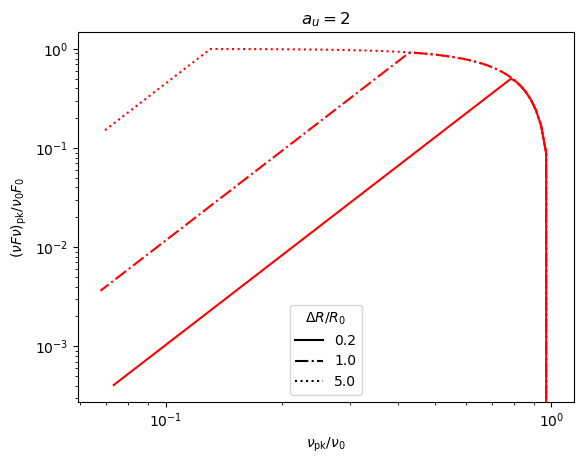
\includegraphics[width=\textwidth]{nupkFnupk_R24b_withdR.png}
% \end{subfigure}
% ~
% \begin{subfigure}{.49\linewidth}
%     \centering
%     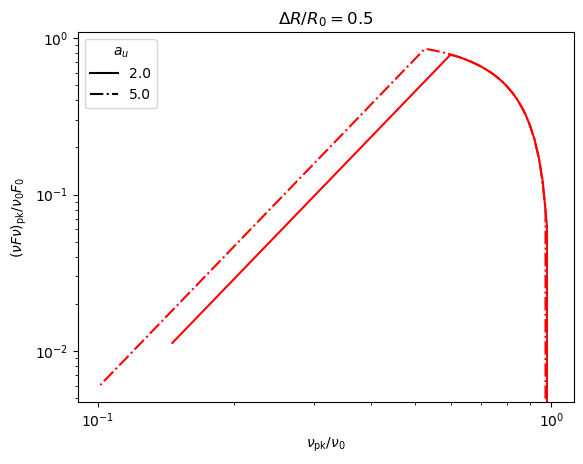
\includegraphics[width=\textwidth]{nupkFnupk_R24b_withau.png}
% \end{subfigure}
% \caption{$\nu_{\rm pk}$ - $(\nu F_\nu)_{\rm pk}$ correlation as predicted by the model. \textbf{Left:} with varying $\Delta R/R_0$ at constant $a_u$. \textbf{Right:} with varying $a_u$ at constant $\Delta R/R_0$.}
% \label{fig:R24b}
% \end{figure*}



\bibliographystyle{aa}
\bibliography{biblio}

% \newpage
% \appendix
% \section*{The python script}
% \lstinputlisting[language=Python]{peak_modeling.py}

\end{document}
